\documentclass[12pt]{article}
\usepackage[margin=.6in]{geometry}
\usepackage{amsmath,amsfonts,amssymb,mathtools}
\usepackage{enumerate}
\usepackage{physics}
\usepackage{graphics,graphicx,epstopdf}
\usepackage[dvipsnames]{xcolor}
\usepackage{float}
\usepackage{hyperref}
\setlength\parindent{0pt}

\newcommand{\R}{\mathbb{R}}
\newcommand{\N}{\mathbb{N}}
\newcommand{\Z}{\mathbb{Z}}
\newcommand{\T}{\mathbb{T}}
\newcommand{\Q}{\mathbb{Q}}
\newcommand{\D}{\mathbb{D}}
\newcommand{\e}{\mathrm{e}}
\newcommand{\C}{\mathbb{C}}

\newcommand{\figlabel}[1]{\textbf{(#1)}}

\newcommand{\comment}[1]{\textsc{\color[rgb]{1,0,0}#1}}

\title{Principal Component Analysis for Semantic Classification \\ AMATH 582 Final Project}
\author{Benjamin Liu, Kelsey Maass, and Riley Molloy}
\begin{document}

% Title/author/abstract
\maketitle
\bigskip

% Abstract
\abstract{Principal component analysis (PCA) and classification by supervised learning are two popular topics in data science today. In this project, we combine techniques from both areas in order to classify news articles based on their word frequency content. We find that we can accurately classify the data by projecting onto a small subset of principal components, reducing the feature space from nearly $10 \,000$ elements to just four. We also compare results from the traditional and robust PCA formulations, and discuss what additional semantic information can be inferred from our results.}


% Sec 1. Introduction and Overview
\section{Introduction and Overview}
Dimensionality reduction is an important tool in data science, often times revealing low-rank system dynamics or structure while increasing computational efficiency. Principal component analysis is fundamental to many dimensionality reduction techniques, grounded in the power of the singular value decomposition. 

Our project employs the use of PCA to lower the dimensionality of a large dataset of articles published by the British Broadcasting Corporation (BBC), with the aim of classifying them according to five topics: business, sports, entertainment, politics, and technology, - i.e. we look to learn the semantics of each article. This type of analysis is often referred to as ``latent semantic indexing". Each article, considered a single observation, is represented by a vector containing the number of times each of 9635 words is used. Rather than classify the articles on this 9635-dimensional feature space, we instead project onto a subset of the dataset's principal components. 

Since the dataset we use is labeled, this is an instance of supervised learning. We train each of our classification schemes on a subset of the data, and then test our classification results on the remaining data. We utilize four different supervised learning techniques: nearest mean, $k$-nearest neighbors, logistic regression, and neural networks. We examine the classification accuracy achieved by each method and how it varies with the number of principal components used to compose the feature space.  

In addition to the traditional PCA formulation, we also employ a variant known as robust PCA. This technique first approximates the original data matrix as the sum of a low rank matrix and a sparse matrix. In our application, the sparse matrix indicates words which are not important to the structure of the larger dataset, but are prominent in a few articles. With the outliers removed from the system, we expect classification schemes trained on the low rank matrix to yield better results. 

% Sec 2. Theoretical Background
\section{Theoretical Background}

% Principal Component Analysis
\subsection{Principal Component Analysis}
Principal component analysis is a powerful tool for isolating low-dimensional
structure embedded in high-dimensional data. The goal of PCA is to find the best
linear transformation of the data which maximizes the variance in the first principal component direction and in each subsequent orthogonal directions. To perform PCA, we utilize the singular value decomposition, or SVD, 
\begin{align} 
A &= U \Sigma V^*,
\label{eq:svd}
\end{align}
which exists for every matrix $A \in \R^{m \times n}.$ In this decomposition the columns of $U$ represent the principal components, or the unit vectors of the new basis, while the columns of $V$ dictate how each article is expressed in the new basis. The elements of $\Sigma$, the singular values, represent the amount of ``energy" present each principal component, while the number of nonzero singular values reveal the rank of the matrix $A$. For systems where the singular values decay rapidly to zero, $A$ can be approximated by truncating the singular value decomposition. For example, using only the first $r$ principal components, we have
\begin{equation}
A \approx U_r \Sigma_r V_r^*,
\end{equation}
where $U \in \R^{m \times r}$, $\Sigma \in \R^{r \times r}$, and $V \in \R^{n \times r}$. Next we can project the matrix $A$ onto this low-rank space spanned by the first $r$ principal components:
\begin{equation}
U_r^* A = \Sigma_r V_r^*.
\end{equation}

% Robust PCA
\subsection{Robust PCA}
Robust principle component analysis is a variant of PCA which presupposes that the data has low-rank structure, but with an unknown amount of sparse noise. That is, for the data matrix $A$ we assume that 
\begin{equation}  A \approx L + S, \end{equation}
where $L$ has low rank and $S$ is sparse. Finding these two matrices can be formulated as the convex optimization problem
\begin{align}
\min_{L,S} \norm{A-L-S}_{F}^2 + \lambda_1 \norm{L}_* + \lambda_2 \norm{S}_1,
\label{eq:robust_obj}
\end{align}
where $\norm{\cdot}_*$ is the nuclear norm, defined by $\norm{\cdot}_* = \norm{\sigma(\cdot)}_1$, where $\sigma$ maps a matrix to a vector of its singular values. In other words, the nuclear norm of a matrix is the sum of its singular values. In addition, $\norm{\cdot}_1$ is the vectorized $\ell_1$ norm, treating the matrix $S \in \R^{m \times n}$ as the vector$S \in \R^{mn}.$ The parameters $\lambda_1$ and $\lambda_2$ can be tuned to prioritize low rank in $L$ or sparsity in $S.$ We can now choose one of many available methods for convex optimization problems, which we discuss in the next section. 

% Sec 3. Algorithm Implementation and Development
\section{Algorithm Implementation and Development}

% Pre-processing and PCA
\subsection{Pre-processing and PCA}

Our dataset consists of 2225 BBC articles labeled by topic, including business (510), entertainment (386), politics (417), sports (511), and technology (401). The data, collected for a paper presented at the 2006 International Conference on Machine Learning [1], consists of integer word counts for 9635 distinct words subject to the following pre-processing steps:
\newpage
\begin{enumerate}
\item Stemming to identify like-words (e.g. fish, fisher, fishing, fishes)
\item Removal of stop words (common words such as: a, about, am, any, are, etc.)
\item Low-count (less than 3) removal
\end{enumerate}

\noindent We arrange our data into a matrix $A \in \R^{9635 \times 2225}$ such that each row represents a different word (or \emph{feature}), and each column represents a different article. To ensure that longer articles do not disproportionately influence our analysis, we divide each column by its sum to convert word counts to word frequencies. We then divide our data into two sets: $80\%$ of each class is put into our training matrix, and the remaining $20\%$ into the cross validation matrix. Next, we subtract the mean of each row in the training set, which ensures that the first principal component has meaningful content rather than just information about the mean article. Finally, we compute the singular value decomposition of the training matrix. Due to the size of our dataset, we only compute the first 10 principal components, using the MATLAB function {\tt svds}. 

% Robust PCA
\subsection{Robust PCA}
As mentioned previously, many methods of optimizing \eqref{eq:robust_obj} exist. We have chosen to implement a method described in \cite{prox} known as the \emph{alternating direction method of multipliers} (ADMM), or \emph{Douglas Rachford splitting}. The algorithm consists of finding closed form representations of the proximal operators of the nuclear norm and the vectorized 1-norm, and evaluating them iteratively and independently, comparing their results.  We utilize an open-source implementation of the algorithm available {\color{blue} \href{http://stanford.edu/~boyd/admm.html}{here}}. Once the low-rank matrix $L$ of the training set is obtained, we convert word count to word frequencies, shift the data to zero mean, and then compute the svd. 

% Classification Schemes
\subsection{Classification Schemes}

To classify articles in our cross validation set, we first project both datasets onto a subset of the training data's principal components. Next we compare our classification accuracy as we increase the number of principal components used for the following classification methods:

\begin{itemize}
\item \textbf{Nearest Mean:} For the nearest mean method, we first project the training data onto
the first $r$ principal components and calculate the average projection for each class. To classify new articles, we assign the label of the closest mean projection.

\item \textbf{$k$-Nearest Neighbors (KNN):} The $k$-nearest neighbors algorithm classifies new articles by
finding their $k$ nearest neighbors and assigning the label shared by the most neighbors. For our article classification, we let $k = 5$.

\item \textbf{Logistic Regression:} Logistic regression classifies articles by first drawing linear decision
boundaries between the classes (one-vs-all) that maximize the log-likelihood of the probabilities that the training articles belong to their respective classes. The final label is chosen from the class with the highest probability.

\item \textbf{Neural Network:} To classify with neural networks, we first build a network with three
layers: input, hidden, output. We then train the network to minimize a cost function on the training data and assign classes to new articles by choosing the class with the highest output value.

\item \textbf{Support Vector Machines:} The motivation behind the support vector machine algorithm is to find a linear decision boundary that maximizes the margin between classes. Data instances that lie along this margin are known as the support vectors. This algorithm works best when data is linearly separable, i.e. no data points cross the decision boundary, but the formulation can be relaxed when this is not the case, penalizing points lying on the wrong side more heavily. Of all our classification methods, we had the most difficulty implementing a support vector machine classifier, which we discuss in detail in the next section.
\end{itemize}

% Sec 4. Computational Results
\section{Computational Results}

% Classification
\subsection{Classification}
In the four classification methods we successfully implemented, we found that the classification accuracy did not significantly increase when we added more than four principal components. We also note that for all of our methods we are able to successfully classify a high percentage of the articles, up to $96\%$ using only four principal components. Surprisingly, the robust formulation does not improve classification accuracy, and in fact sometimes performs slightly worse. Unfortunately we were not able to tune the robust PCA parameters to see if we could improve results, due to the expense of the factorization algorithm. 

\begin{table}[H]
\begin{minipage}{0.5\textwidth}
\begin{center}\textbf{PCA}\end{center}
\begin{tabular}{c | c | c | c | c | c}
 {\bf Rank } & {\bf 1 } & {\bf 2} & {\bf 3} & {\bf 4} & {\bf 5 } \\ \hline
Nearest Mean & 59\% & 77\% & 82\% & 96\%  & 96\% \\
KNN ($K = 5$) & 56\% & 77\% & 86\% & 96\%  & 97\% \\
Logistic & 45\% & 75\% & 78\% & 94\%  & 94\% \\
Neural Net & 46\% & 75\% & 79\% & 95\%  & 95\%
\end{tabular}
\end{minipage}
\begin{minipage}{0.5\textwidth}
\begin{center}\textbf{Robust PCA}\end{center}
\begin{tabular}{c | c | c | c | c | c}
 {\bf Rank } & {\bf 1 } & {\bf 2} & {\bf 3} & {\bf 4} & {\bf 5 } \\ \hline
Nearest Mean & 48\% & 78\% & 89\% & 95\%  & 96\% \\
KNN ($K = 5$) & 52\% & 77\% & 92\% & 96\%  & 96\% \\
Logistic & 45\% & 74\% & 77\% & 93\%  & 93\% \\
Neural Net & 45\% & 74\% & 79\% & 93\%  & 93\%
\end{tabular}
\end{minipage}
\caption{Comparison of classification accuracy for as we vary rank for our four classification algorithms on the traditional PCA space (left) and robust PCA space (right).}
\end{table}

\begin{figure}[H]
\centering
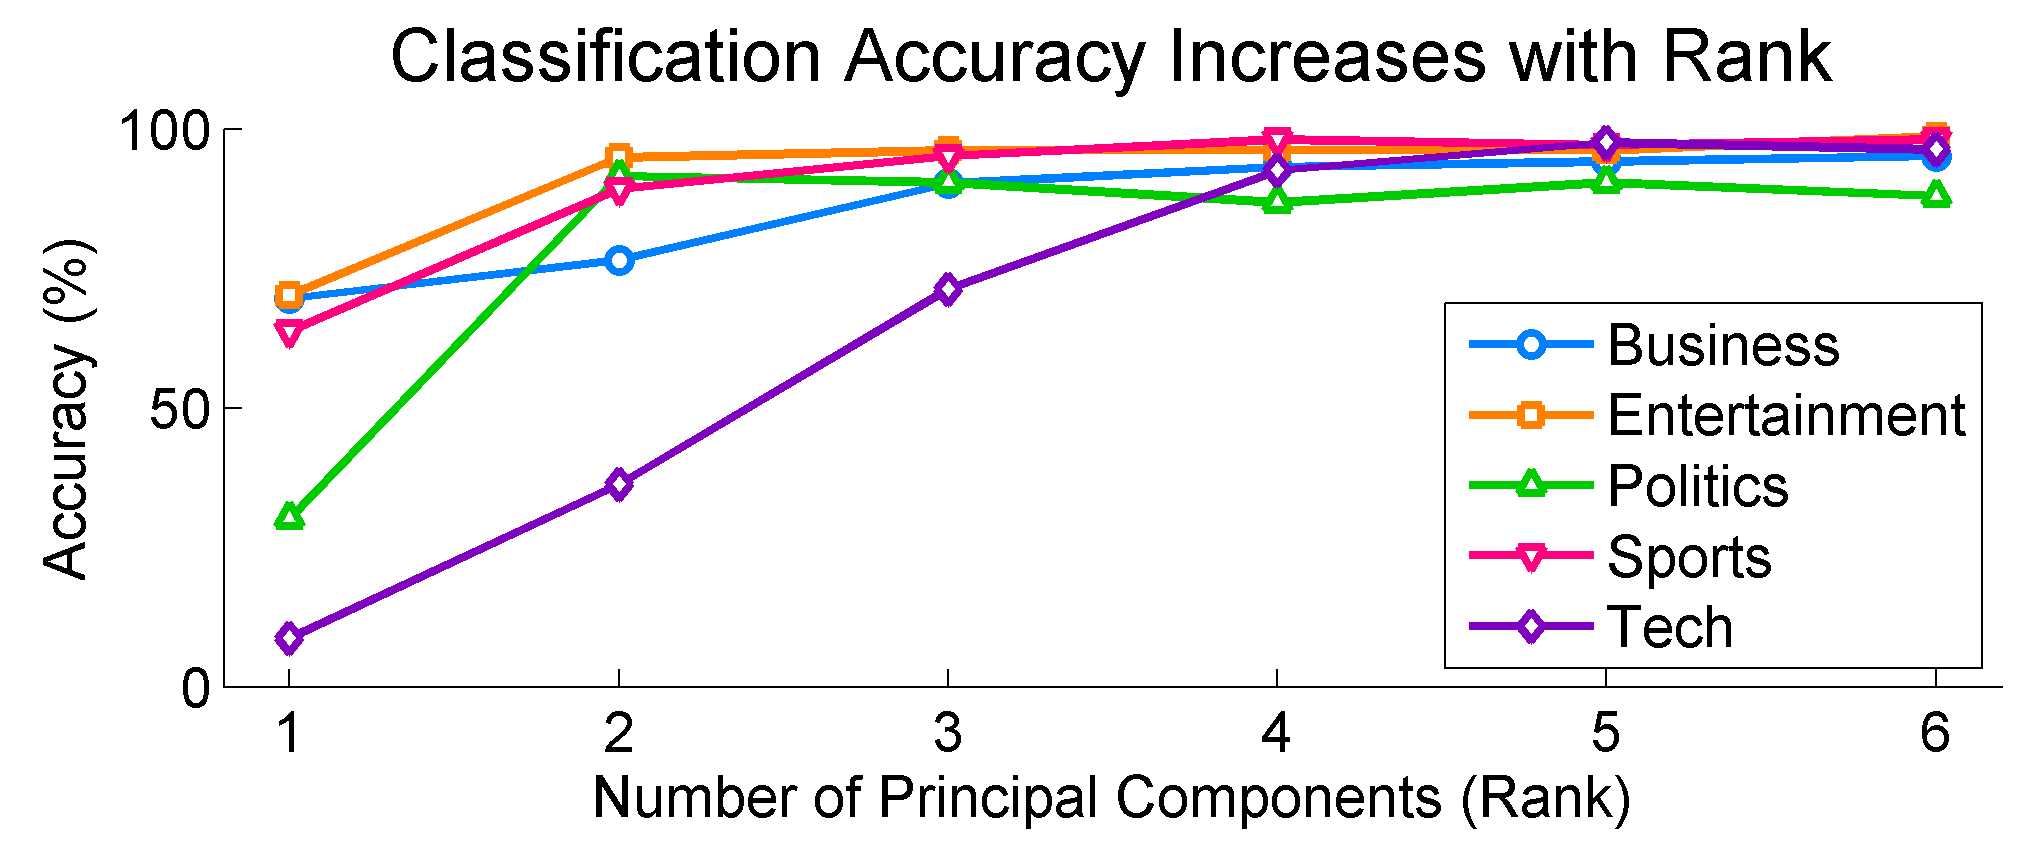
\includegraphics[width=.6\textwidth]{figures/accuracybyrank}
\caption{Comparison of classification accuracy for $k$-nearest neighbors ($k = 5$) for each article class as we vary the number of principal components used.}
\label{class_accuracy}
\end{figure}

To understand why increasing the number of principal components does not significantly improve classification accuracy, we look at how each article class is expressed in the principal component basis. In Figure 2 we plot the column vectors of $V$, which express how each article is projected onto the principal components. We note that the articles are differentiated by class in the first four principal components, but not in the fifth. This is also true for principal components 6-10. This illustrates the fact that while using a higher-rank matrix might better approximate the data, only the first four significantly contribute to the task of classification. Furthermore, Figure 1 seems to suggest that only the first three principal components are necessary to classify the first four categories, while the fourth principal component is needed for correctly classifying the tech articles. In fact, if we look at the expression of the tech articles in Figure 2, at least for the traditional PCA results, we see that the tech articles are only differentiated by the fourth principal component. 

\begin{figure}[H]
\centering
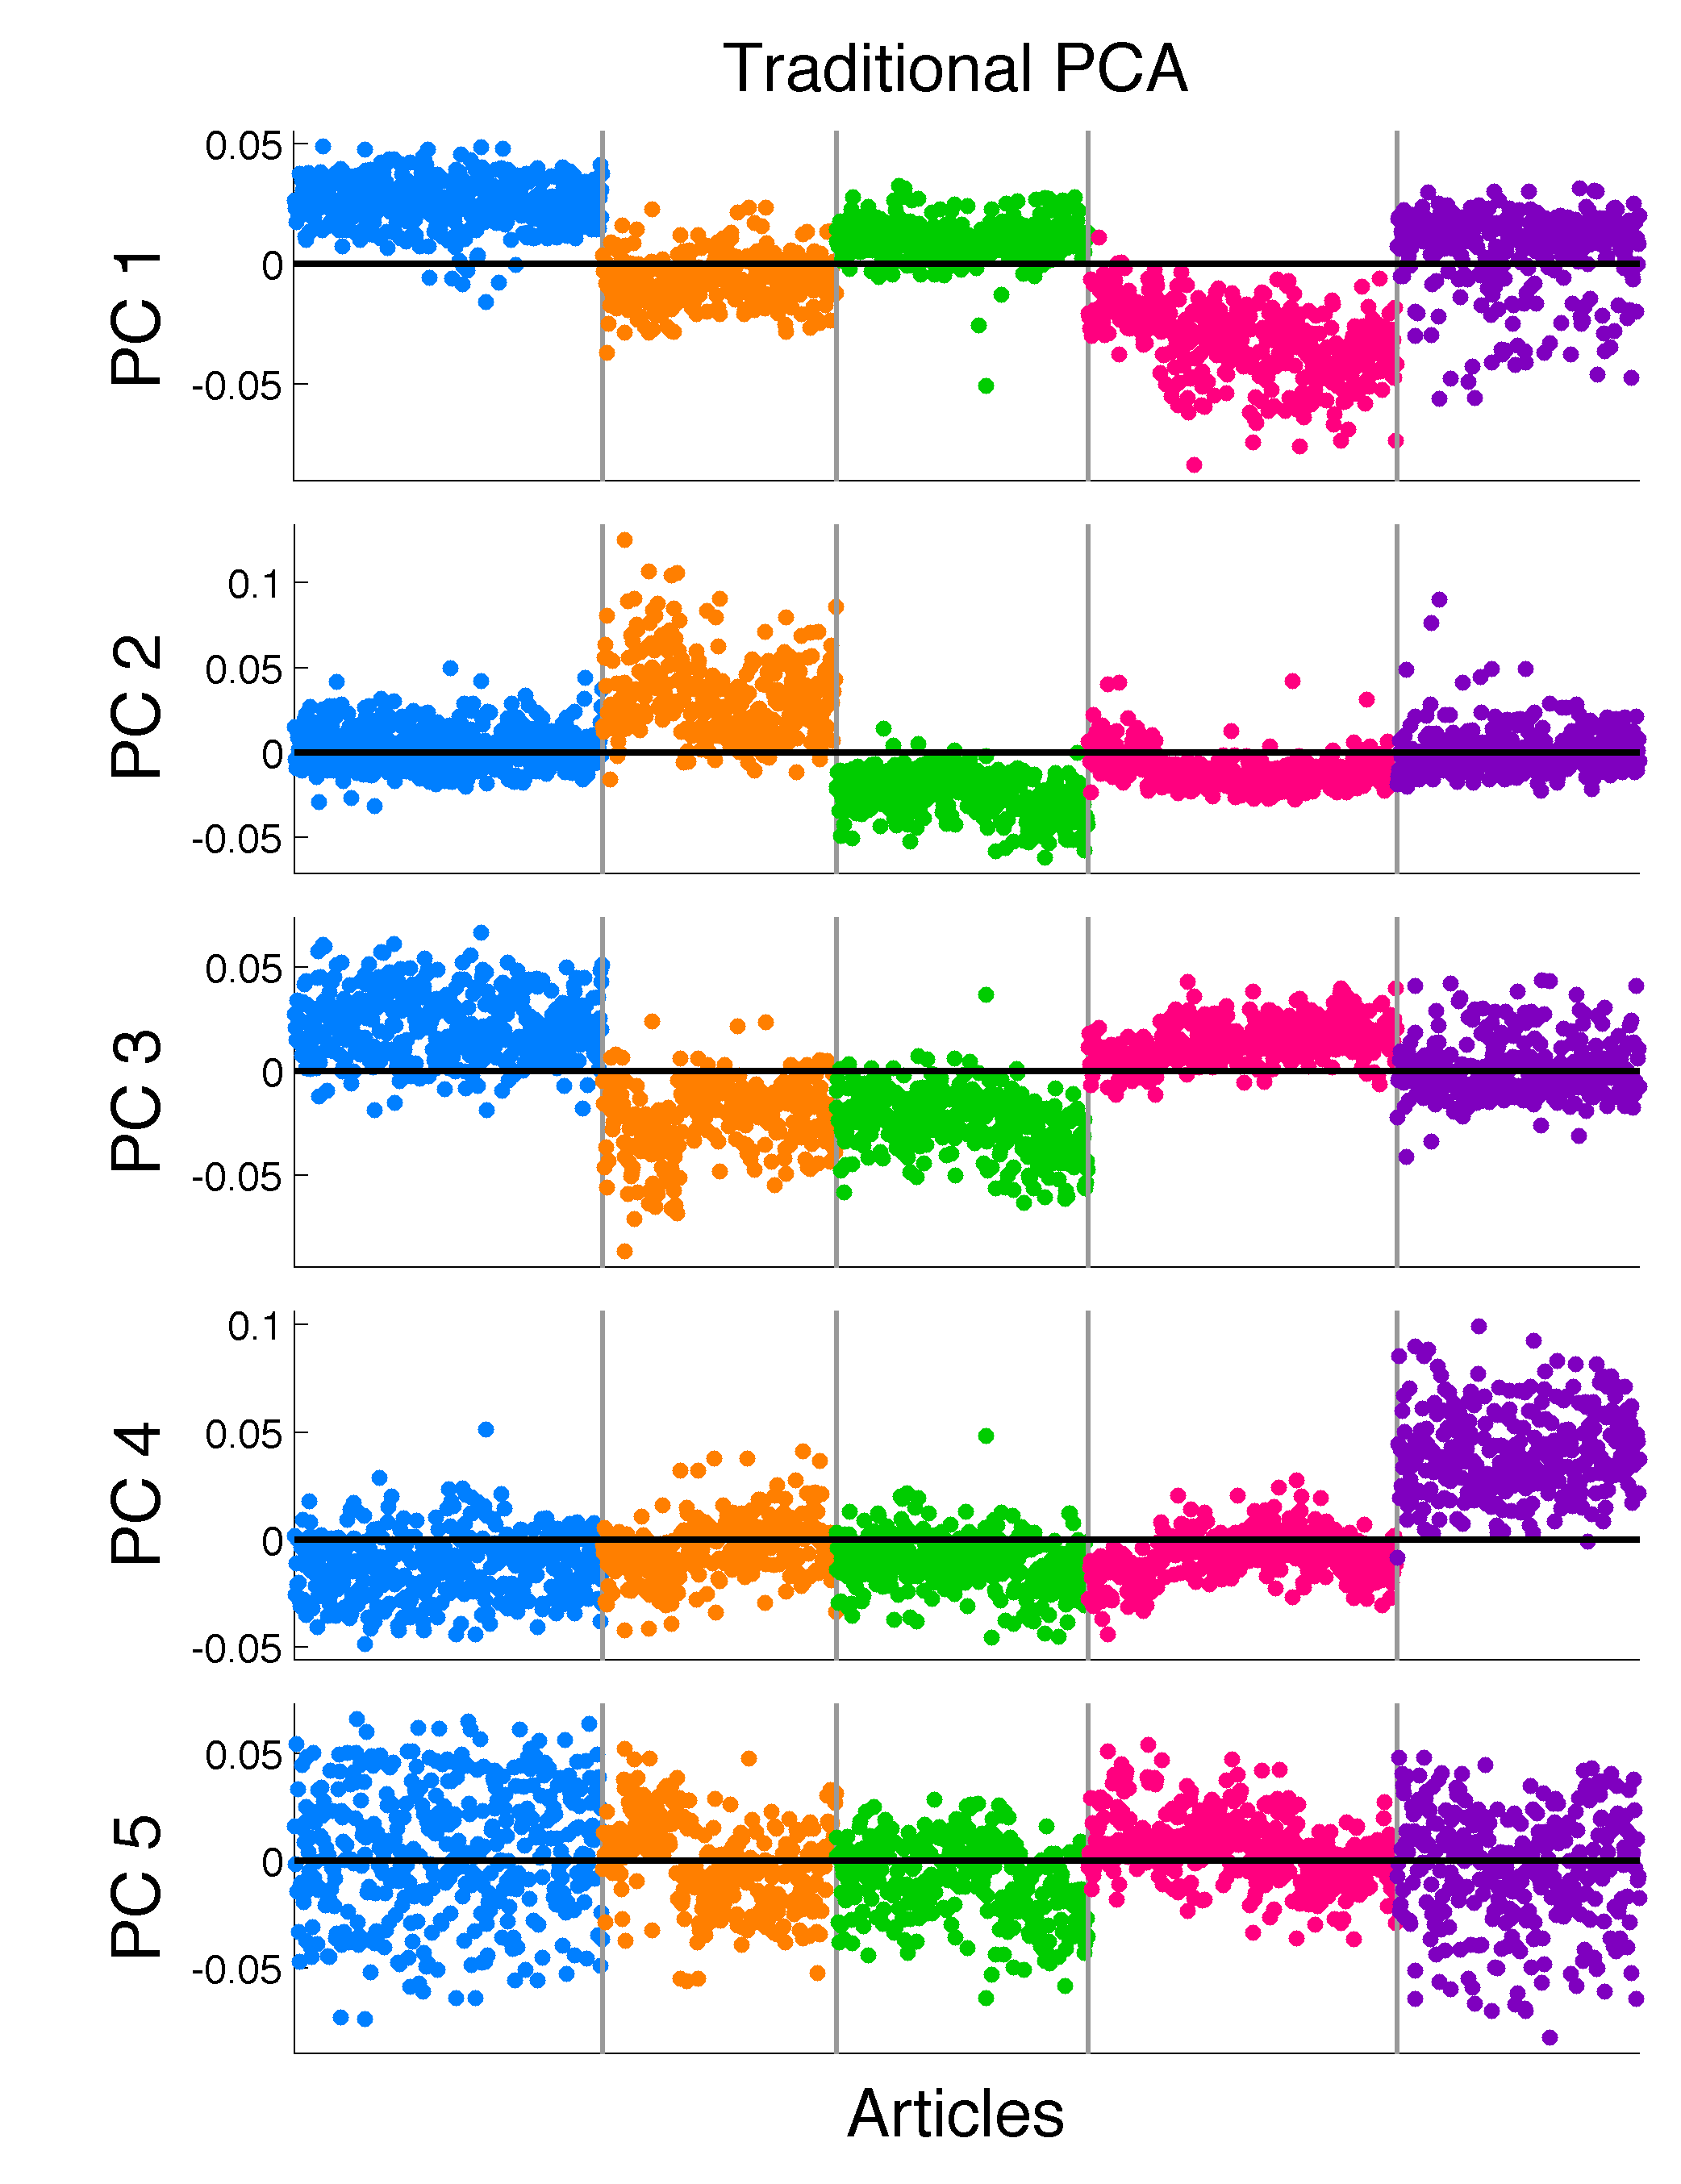
\includegraphics[width=3in]{figures/principalcomponents_original} \quad
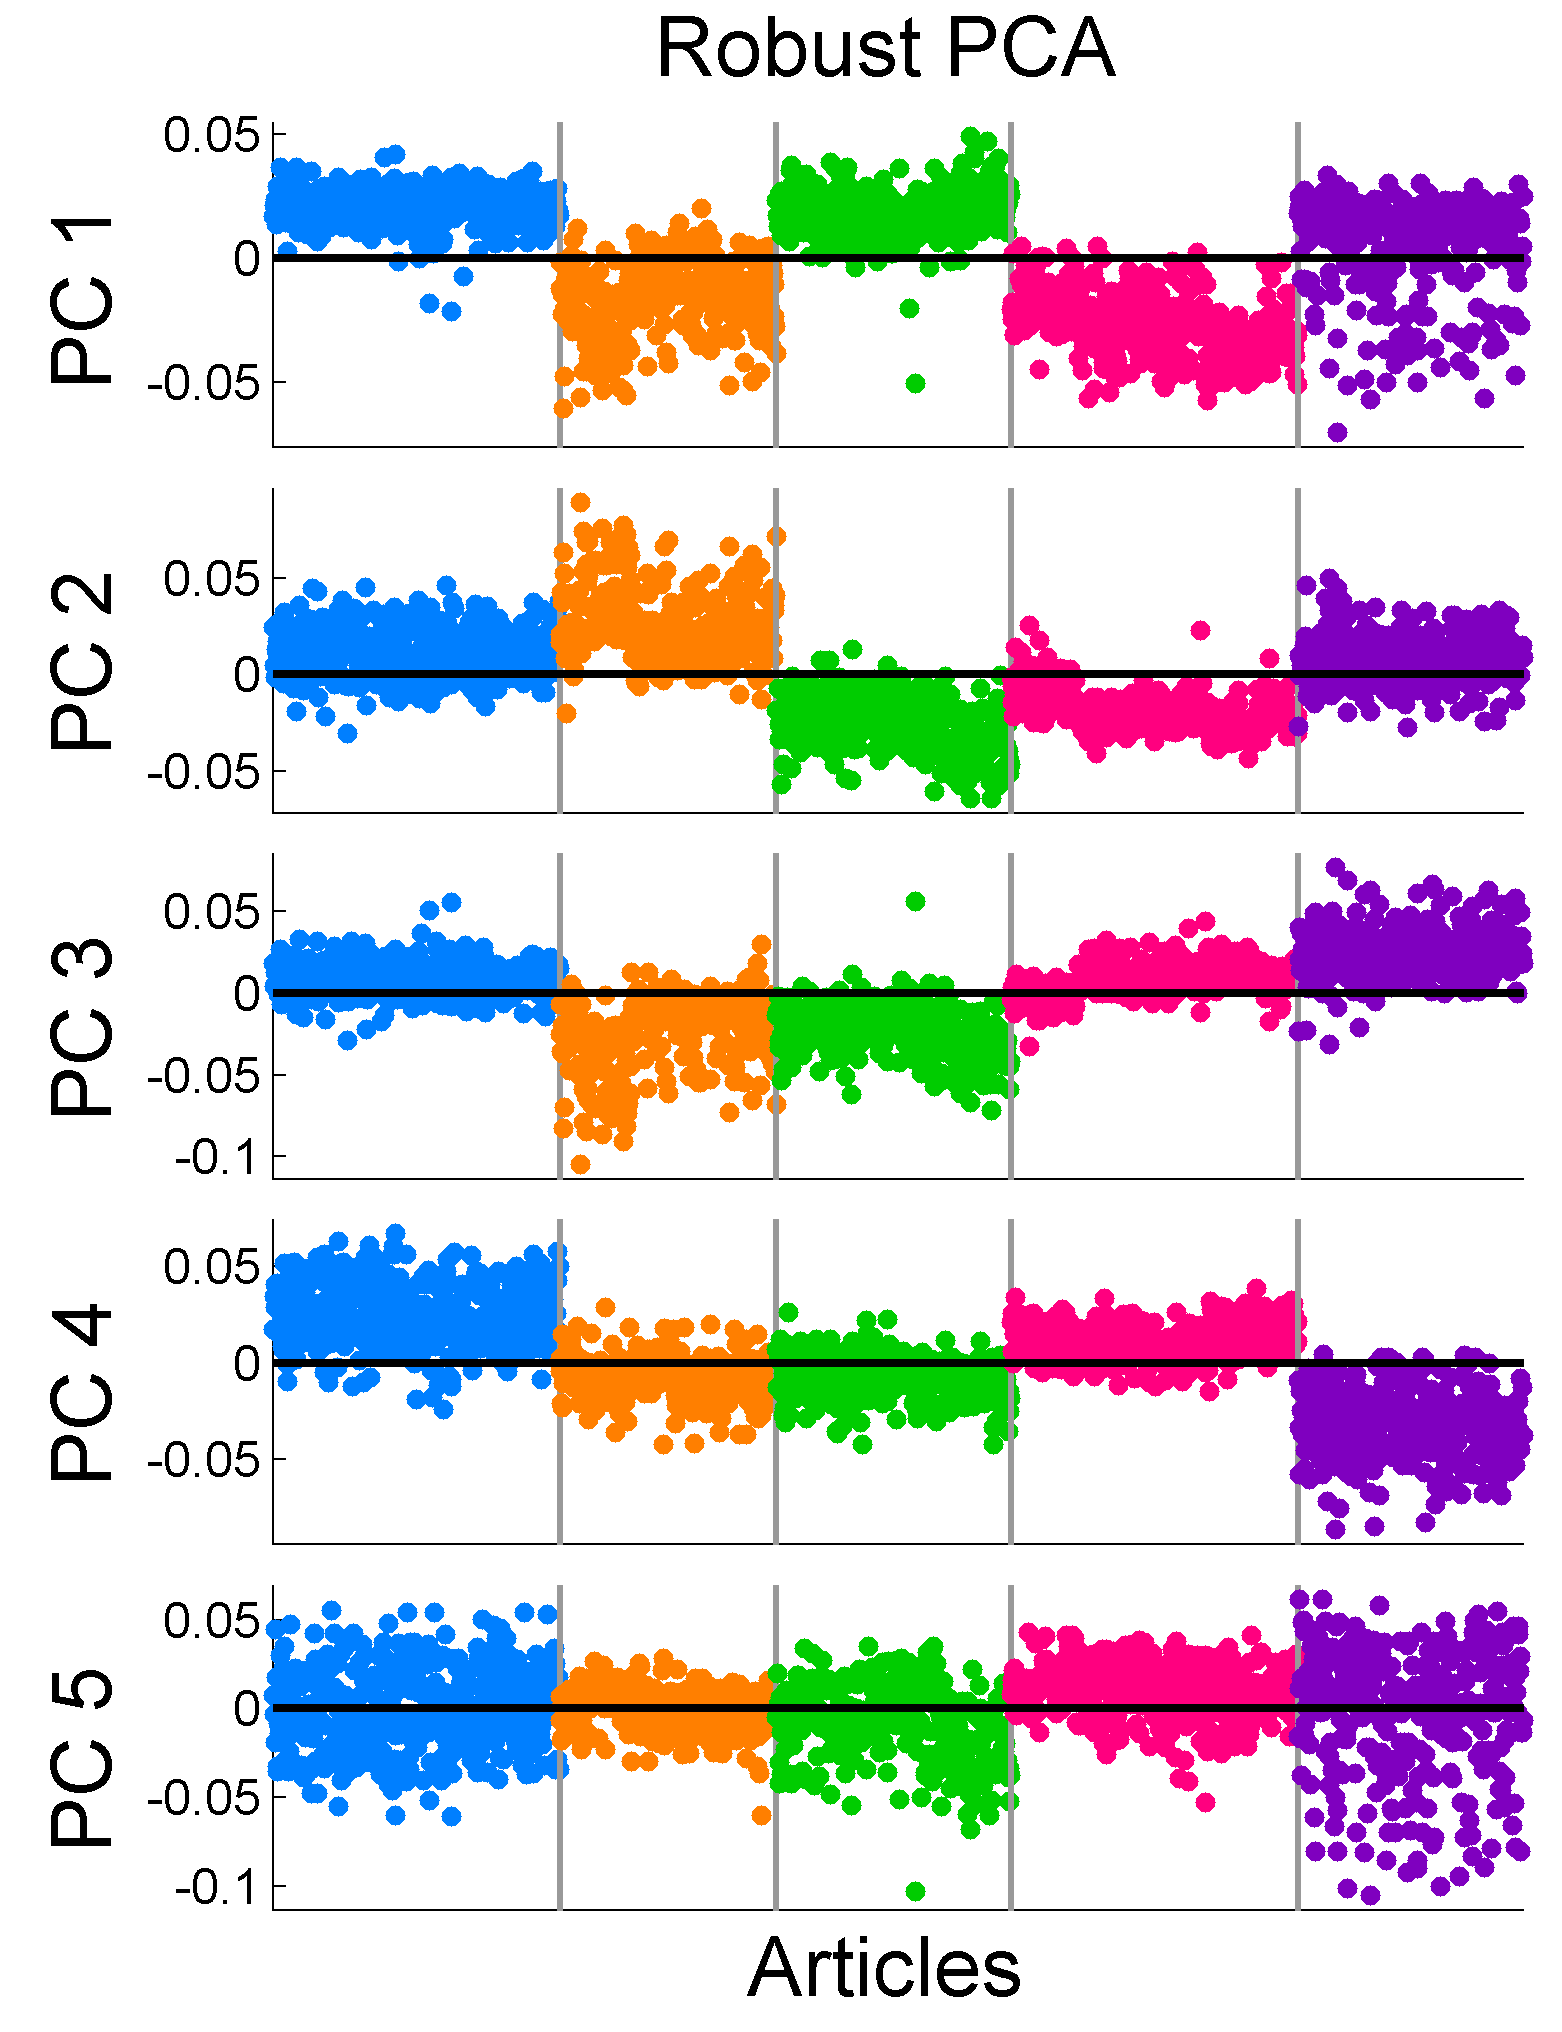
\includegraphics[width=3in]{figures/principalcomponents_robust}
\caption{Visualization of the columns of $V$, which illustrate how each article is projected onto each of the first five principal components. We note that while the articles are differentiated by class in the first four principal components, they are not with the fifth. }
\end{figure}

We can also look at the singular values of the data matrix to determine how important each principal component is for representing the system. In Figure \ref{sing_val} below, we compare the energy percentages of each of the first 100 singular values for both the traditional PCA and robust PCA formulations, where we note that the first four principal components increase in significance for robust PCA. It is therefore surprising that robust PCA performed worse in our classification schemes! 

\begin{figure}[H]
\centering
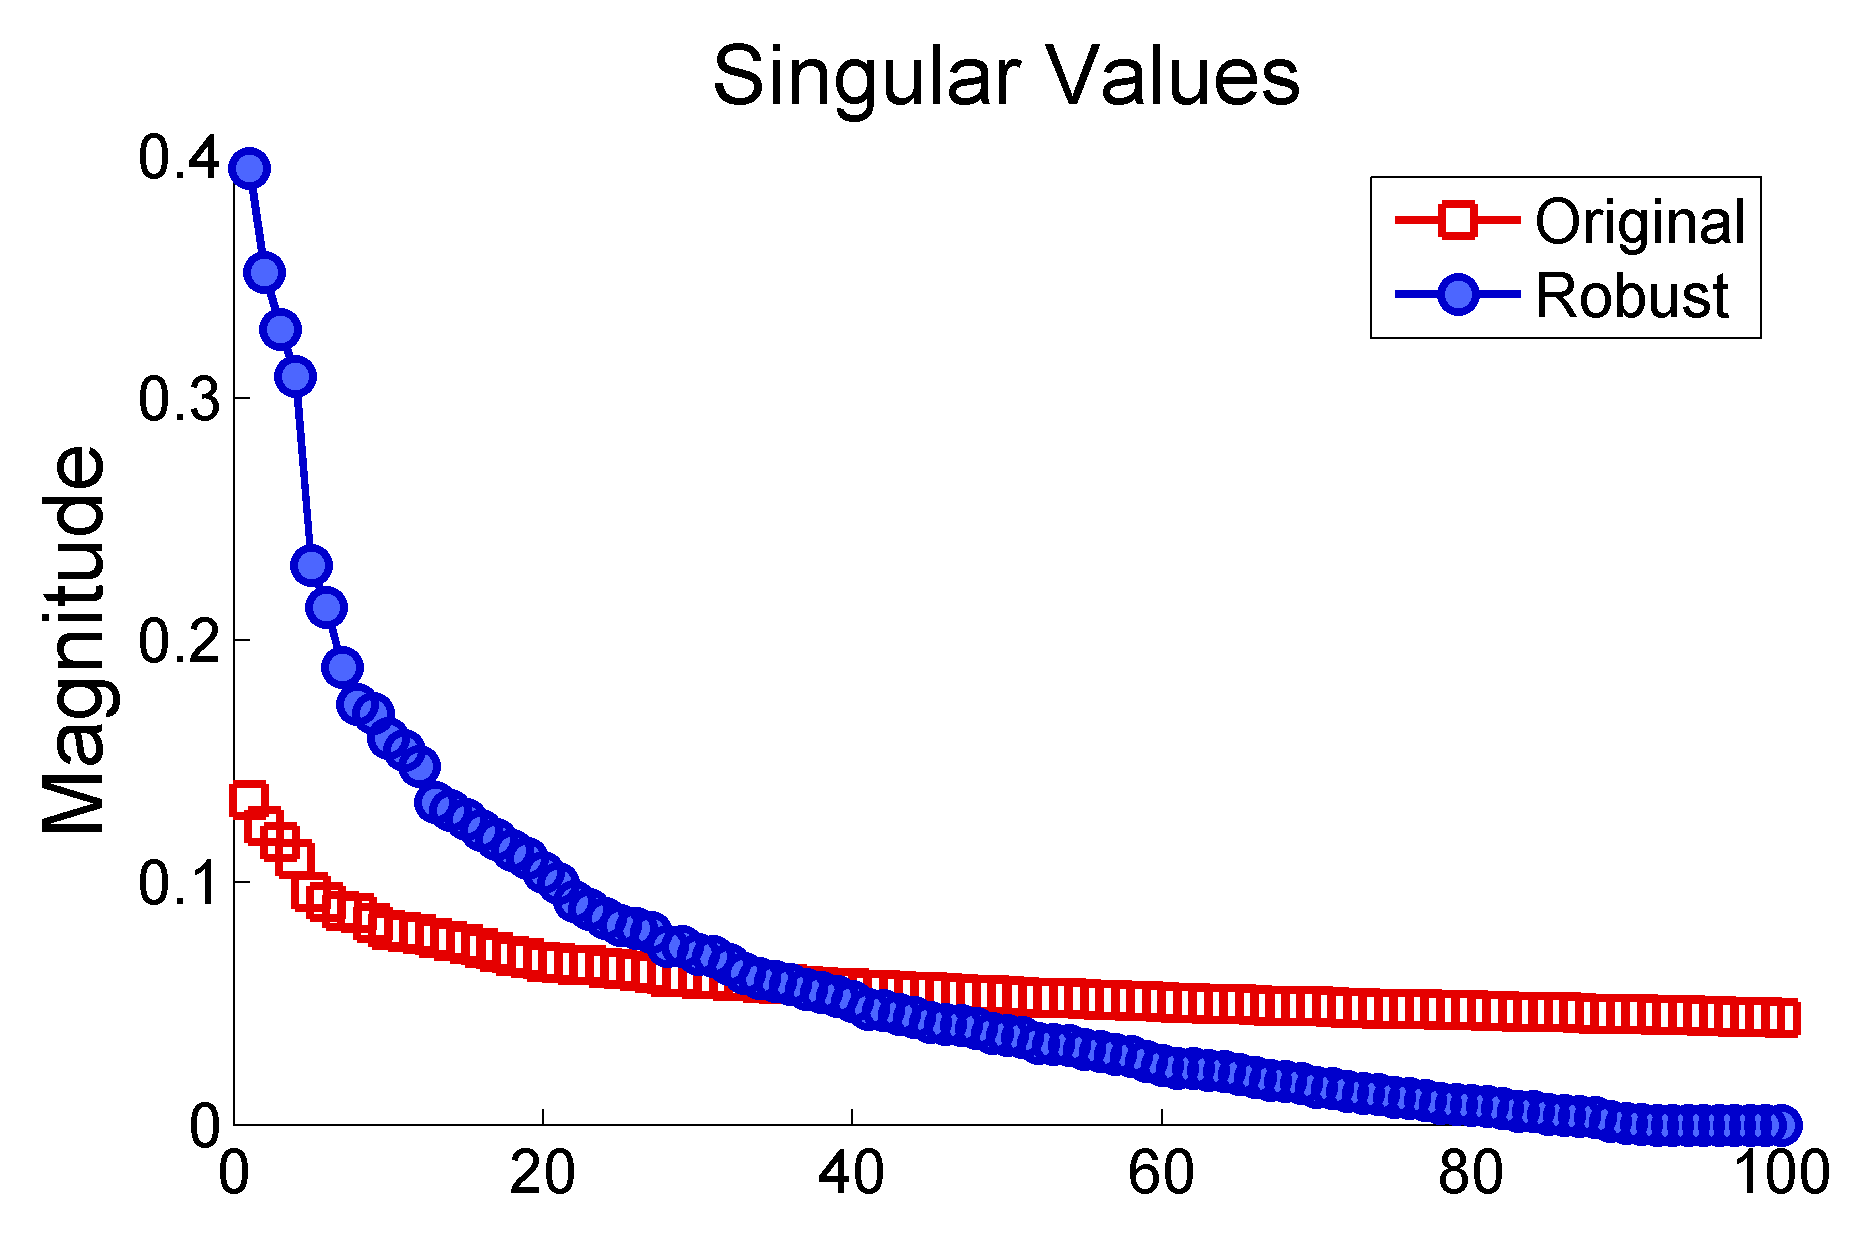
\includegraphics[width=.6\textwidth]{figures/singularvaluescompare}
\caption{Comparison of first 100 singular values derived from the data with traditional and robust PCA formulations. The singular values are normalized by the Frobenius norm of each data matrix. }
\label{sing_val}
\end{figure}


% Misclassification
\subsubsection{Misclassification}
While projecting onto the principal components of the training set does a good job at separating the article by class, it does
not separate them perfectly. Therefore articles near the decision boundaries may be misclassified.

For example, Figure \ref{misclassification} shows how articles from each class are classified by the $k$-nearest neighbor algorithm as we vary the number of principal components used. It is interesting to note that articles from business and politics are likely to be mistakenly cross-classified. Furthermore, technology articles are prone to misclassification if the fourth principal component, which contains many technology-related words, is ignored.

\begin{figure}[H]
\centering
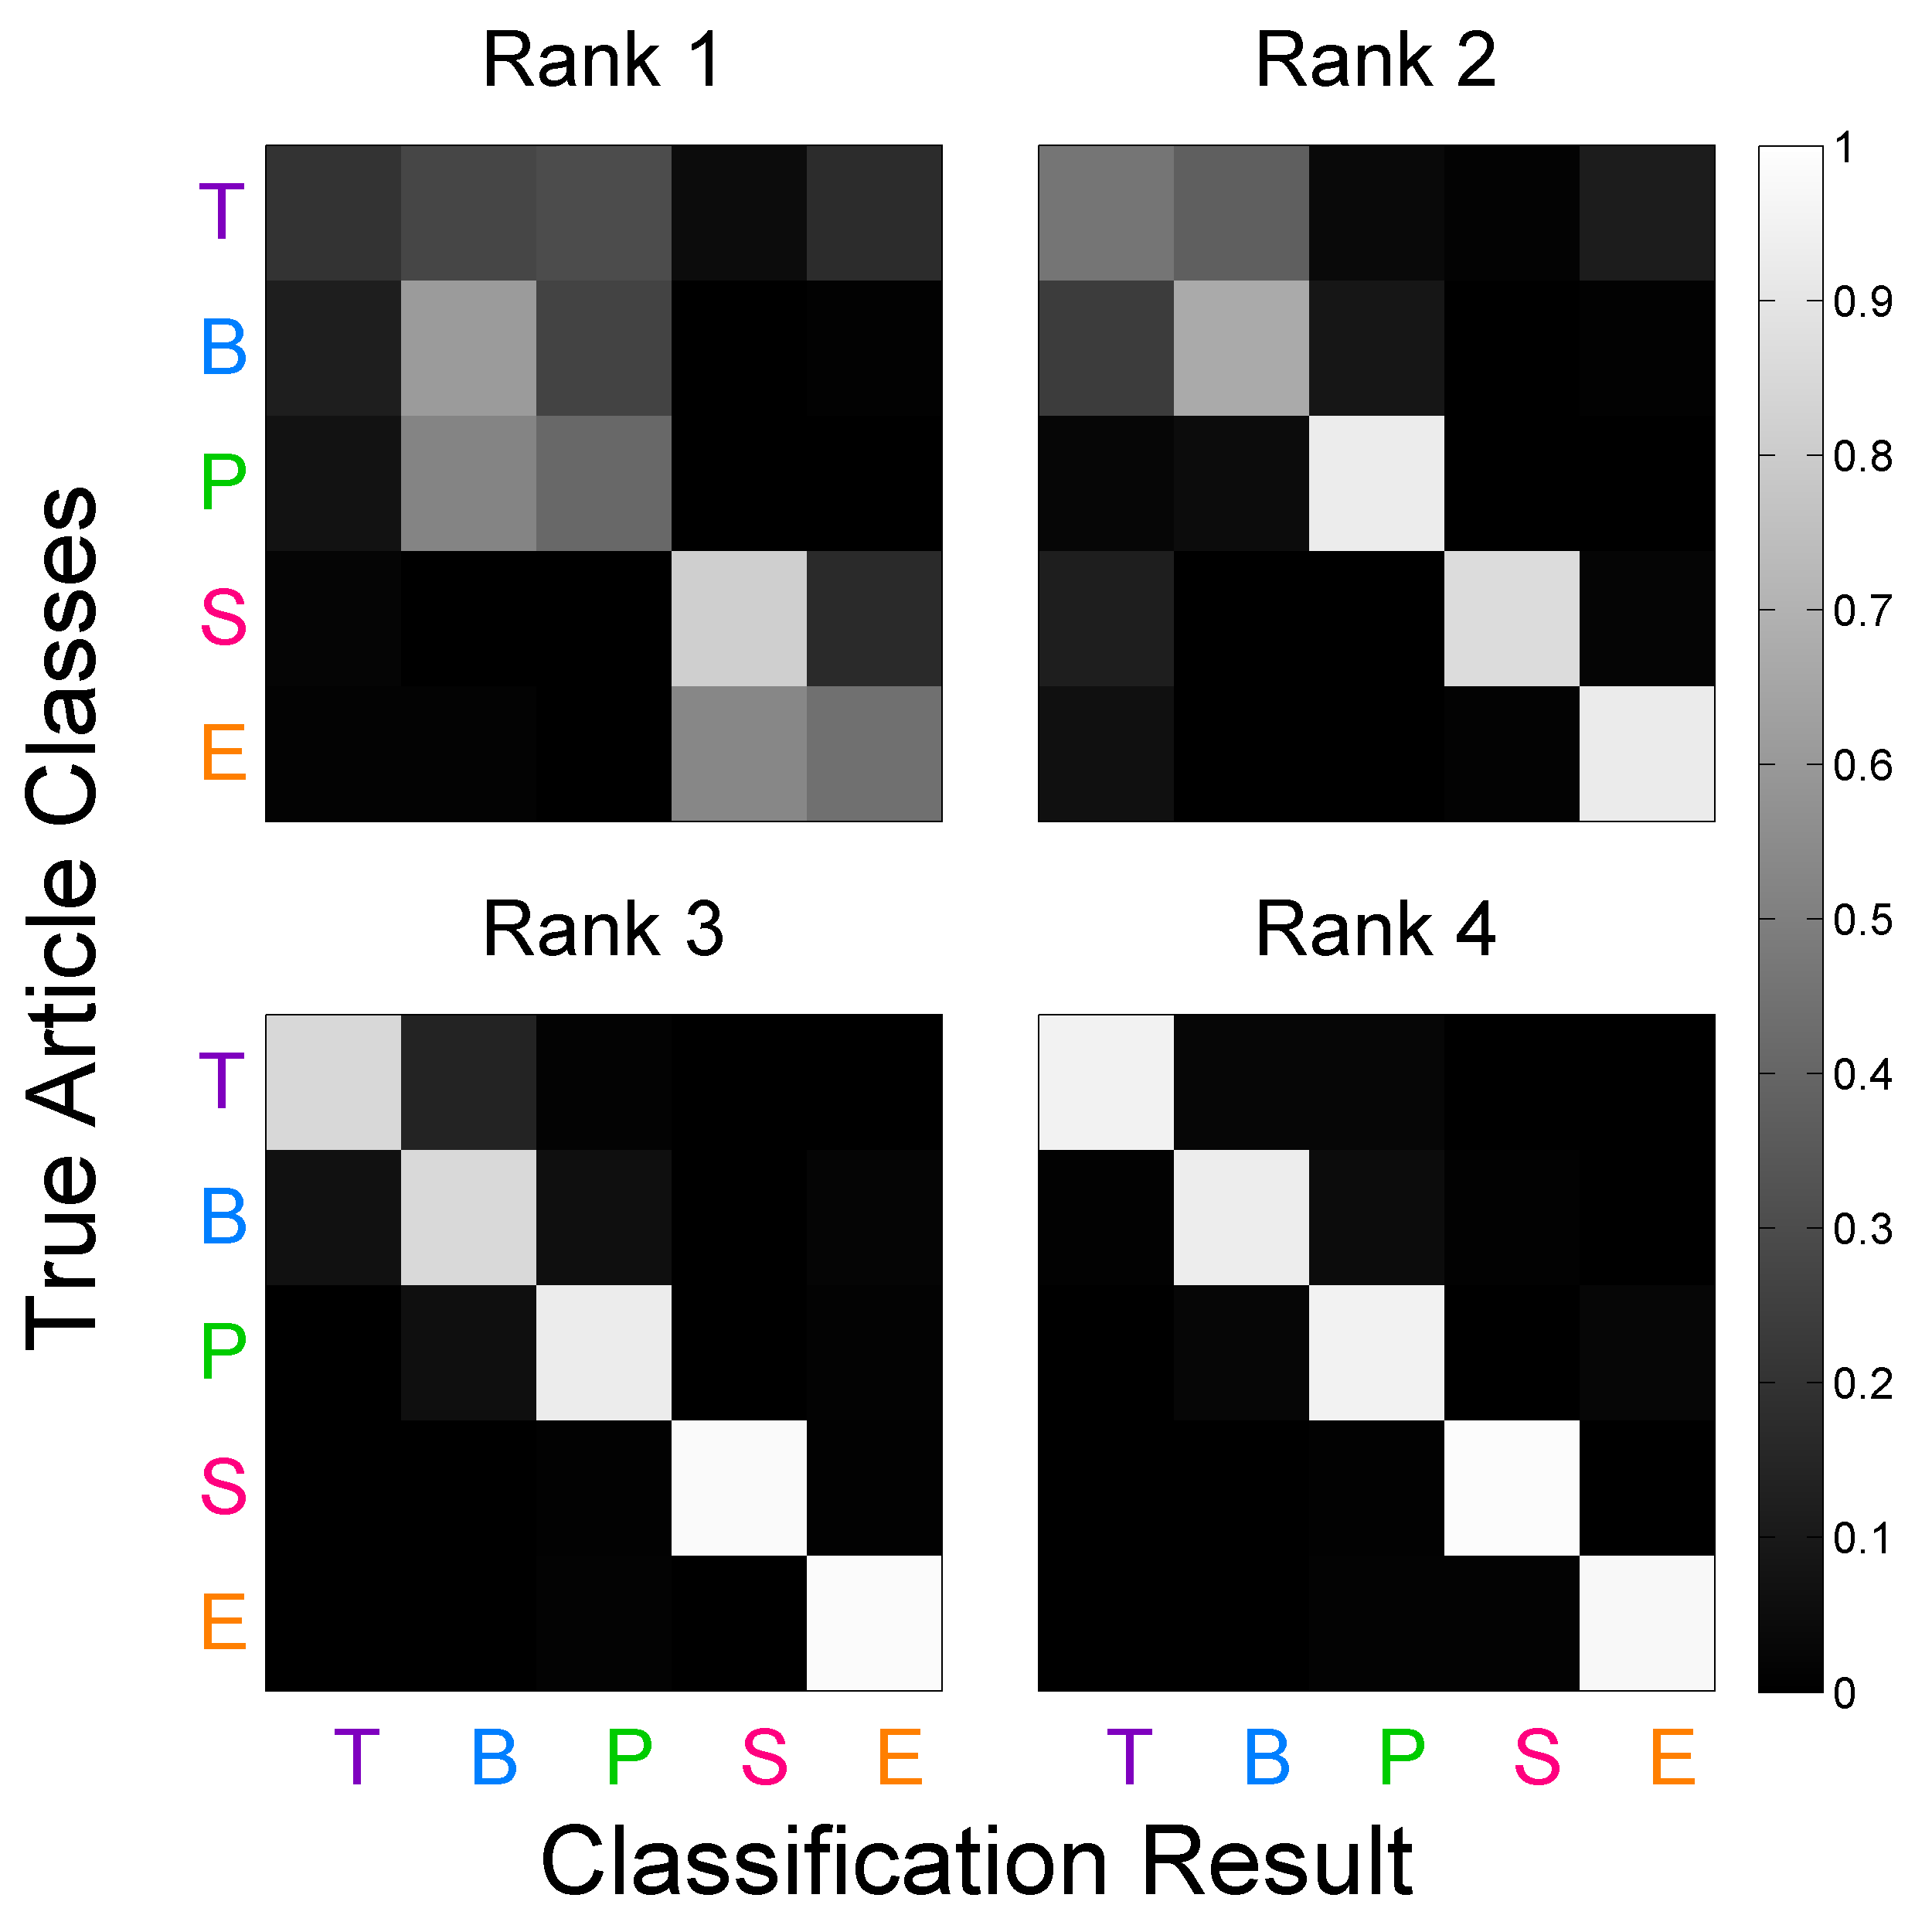
\includegraphics[scale=.5]{figures/classificationmatrices}
\caption{Classification of each article by type. Diagonal elements indicate percent of articles classified correctly; off-diagonal
elements correspond to misclassified articles.}
\label{misclassification}
\end{figure}

% Neural Networks
\subsubsection{Issues: Neural Network}

Another surprising result we encountered was the fact that the classification accuracy of the neural network algorithm was better for the cross validation set than for the training set, which is highly unusual. This result is illustrated in Figure 5 below. One explanation could be that in our particular data partitioning there were more outliers in the training data than in the cross validation data. Another reason could be that we needed to adjust our regularization parameter in the neural network formulation. We also note that the traditional PCA seems to be \emph{less} sensitive to changes in the number of principal components used than the robust formulation. However, this may be due in part to the fact that the weight vectors are initialized randomly, so each run can yield slightly different results. 

\begin{figure}[H]
\centering
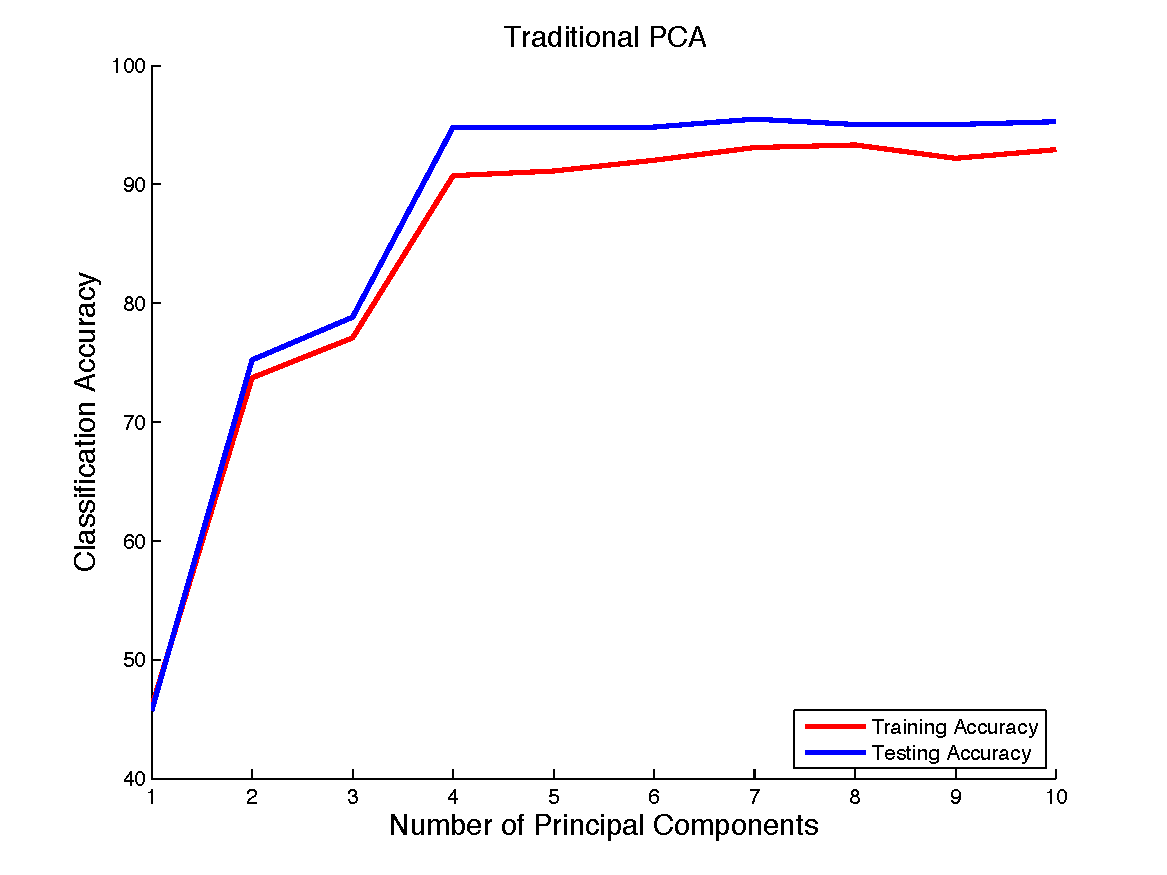
\includegraphics[width=3in]{figures/nn_trad} \quad
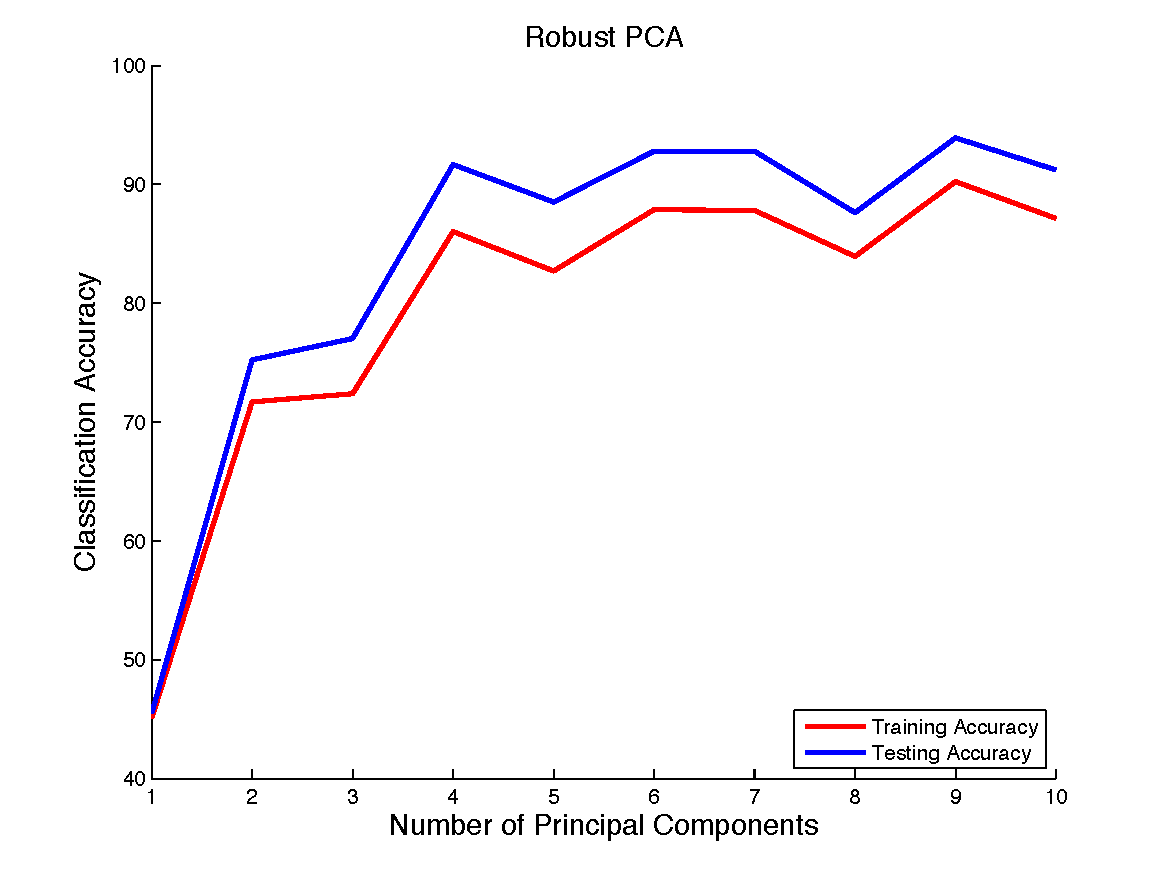
\includegraphics[width=3in]{figures/nn_robust}
\caption{Classification accuracy on the training and cross validation datasets obtained using a neural network. Accuracy increases as we include more principal components, and levels off after four principal components are added. However, the robust PCA results experience fluctuations as we vary the number of principal components used.}
\end{figure}


% Support Vector Machines
\subsubsection{Issues: Support Vector Machine}

Support vector machines (SVMs) are, in their basis formulation, binary classifiers. This means that they can only classify data between two classes. Several approaches exist to extend the SVM framework to support classification between more than two classes, such as one-versus-all, where SVMs are built to classify each class against all others, and one-versus-one, where SVMs are built to classify each class against each other class.

Simply generating multiple SVMs does not immediately fix the problem. Figure \ref{fig:svm_training} shows results from applying the one-versus-all support vector machine classification scheme on data from four classes. Though the four classes are quite well-separated in space, attempting to separate each class against the remaining three with a linear separator is not very successful; data points in the central region are negatively classified by all of the support vector machines, whereas data points in the top, bottom, left, and right regions are doubly-classified.
\begin{figure}[H]
\centering
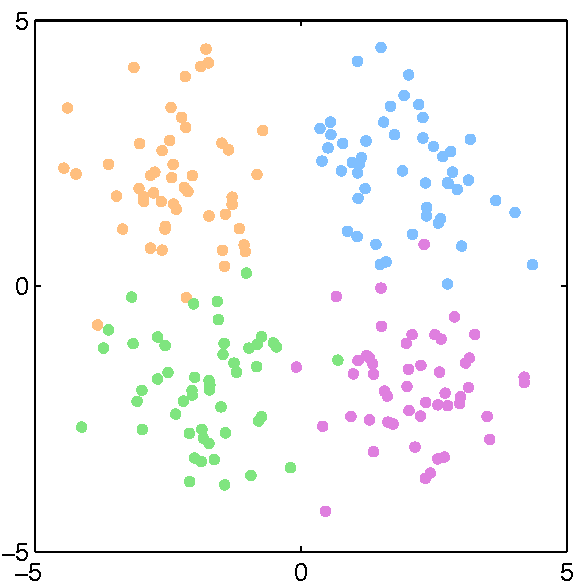
\includegraphics[width=.4\textwidth]{figures/svm_trainingdata}
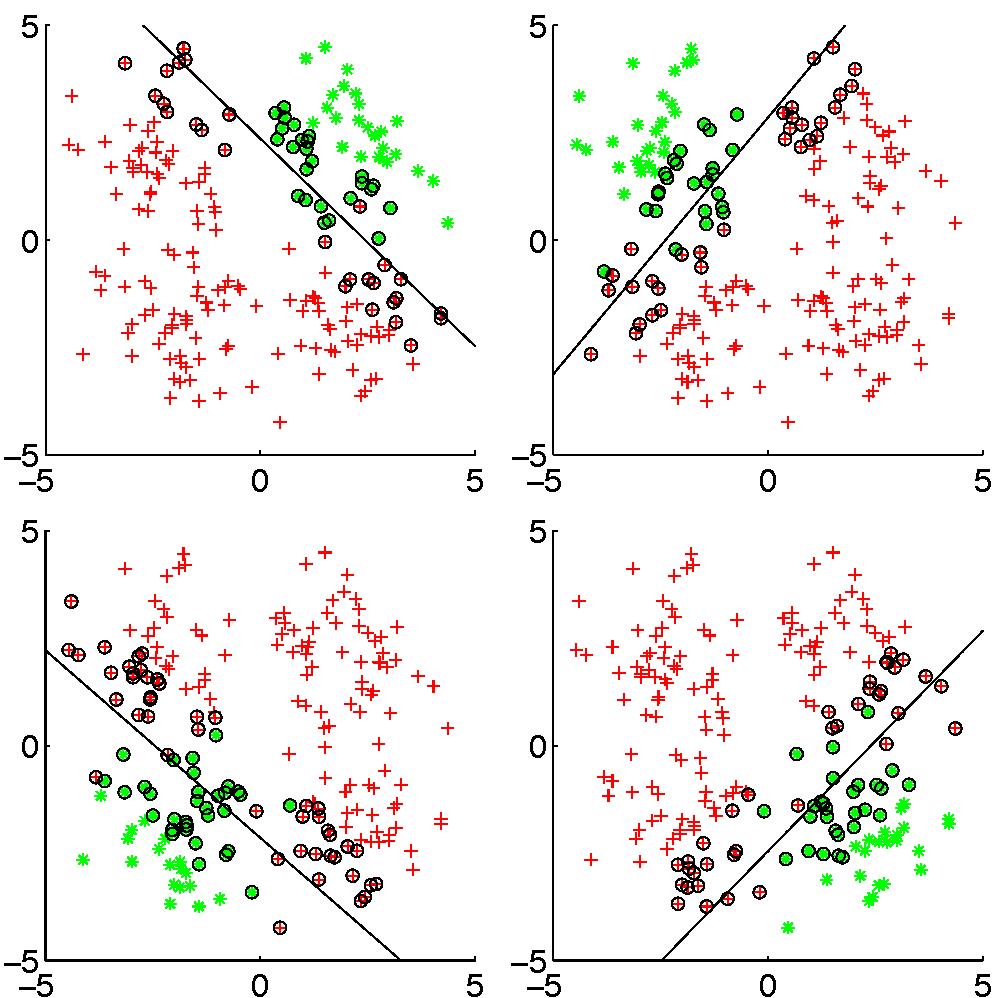
\includegraphics[width=.4\textwidth]{figures/svm_multiplesvms}
\caption{One-versus-all scheme for classification by support vector machine into four classes. \figlabel{Left} Training data from four classes with some overlap. \figlabel{Right} Support vector machines generated by considering data from each class versus all others.}
\label{fig:svm_training}
\end{figure}
To truly extend the one-versus-all SVM framework to classify multiple classes, we modify the SVM formalism so that rather than giving a binary classification, it provides a measure of goodness of fit. This can be thought of as returning the (signed) distance of the data point to the decision boundary, rather than simply which side of the decision boundary it falls on. We then compare the results of classifying the data point with each of the SVMs, and choose the SVM which classifies the data point as `deepest' within the positive decision region. Figure \ref{fig:svm_classify} shows the result of applying this classification scheme on the data from Figure \ref{fig:svm_training} with new test data points. 
\begin{figure}[H]
\centering
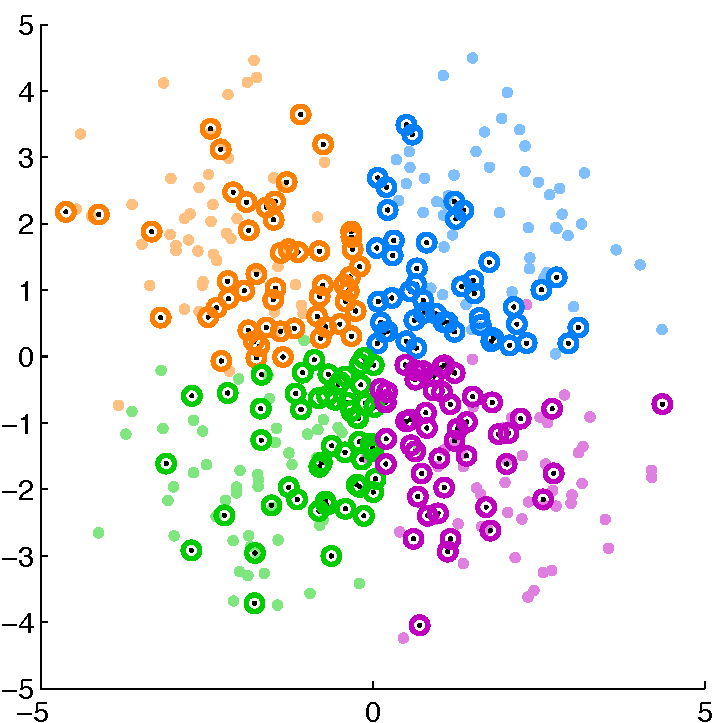
\includegraphics[width=.48\textwidth]{figures/svm_classification}
\caption{Results from applying the one-versus-all SVM classification scheme to test data. Classifications are shown as circles around each point.}
\label{fig:svm_classify}
\end{figure}

In our work with the BBC article data, we found that the built-in optimization routines used in building the SVMs failed to converge for the large data set. We found that even in our two-dimensional test cases, that by increasing the number of data points in the training set we could induce this problem. It therefore seems that isolating the support vector training data points may have been the most significant factor in algorithm convergence, and we speculate that performing some kind of pre-processing to remove easily-classified (interior) points in each class may improve the performance of the algorithm.

% PCA and Robust PCA
\subsection{Semantic Analysis}

While data methods are powerful tools for discovering trends and structure in large datasets, inferring semantic meaning from these models can be difficult. For example, principal component analysis determines the best basis to represent our article data in terms of word frequency values and variance, with no regard to semantic meaning. Nevertheless, our article classification analysis uncovers some trends with meaningful interpretation in terms of the thematic content of the articles.

Below, we list the 25 words with the highest weights in each of the first four principal components. Since each principal component is a linear combination of words, it is difficult to interpret their meaning. However, we note that the fourth principal
component has many technology-related words, which could explain why the inclusion of the fourth principal component is necessary to correctly classify technology articles.

\newpage
\begin{itemize}
\item {\bf PC 1:} game, play, win, player, firm, England, company, market, govern, year, against, team, growth, share, side, best, sale, price, club, bank, economy, go, cup, people, coach
\item {\bf PC 2:} film, award, year, best, music, party, labour, star, elect, govern, Blair, include, sale, ministry, Tori, top, show, actor, nomination, told, number, album, 2004, people, band
\item {\bf PC 3:}  film, game, party, sale, labour, year, best, award, elect, market, firm, Blair, people, company, growth, price, share, Tori, profit, bank, music, ministry, England, star, player
\item {\bf PC 4:} people, game, phone, user, mobile, year, tech, music, service, software, Microsoft, computer, firm, best, site, program, govern, search, labour, economy, elect, digital,
net, online, Blair
\end{itemize}

\subsubsection{Sparse Matrix Analysis}
Robust PCA yields a sparse matrix containing elements which represent words important to a small number of articles. Our sparse matrix contained 252 non-zero elements, compared with 227,814, the total number of non-zero elements in the training dataset. We notice that these words correspond to subtopics within given category (e.g.: last names of athletes, music terminology, “Yahoo”). Some of the most frequent of these words are listed below.

\begin{center}
\begin{tabular}{c c c c c}
{\bf Business} & {\bf Sports} & {\bf Entertainment} & {\bf Politics} & {\bf Tech} \\ \hline
call & roddick & song & wage & game \\
centre & nadal & music & minimum & ink \\
 & dallaglio & urban & forsythe & yahoo \\
 & & best & increase & gadget \\
\end{tabular}
\end{center}





% Sec 5. Summary and Conclusions
\section{Summary and Conclusions}

In our work we sought to classify news articles by category based on their word frequencies. At its core, this is a very high-dimensional problem where objects must be classified based on a large number of features. The number of dimensions is given by the number of words in the articles to be classified, or in a broader sense, the number of words in the common lexicon.

Using principal component analysis we found low-rank structure present in the the article feature space. The true feature space, spanning 9635 dimensions (words) can be re-represented as a four-dimensional space suitable for classification of articles into five distinct categories.  By projecting articles into the principal component space, we achieved high classification accuracy with several classical classification algorithms. While classification based on principal component analysis proved to be very successful, it is difficult to glean any meaning from these analyses. The principal components do not in general correspond to any of the article categories or to any semantic or thematic trends or groups.

In addition to standard principal component analysis, we also performed robust PCA on the data. In terms of classification accuracy, we found that the traditional PCA formulation performs slightly better than the robust PCA formulation. Rather than improving classification, we found that robust PCA can isolate semantically meaningful elements of the data that can be readily interpreted in terms of the themes of the articles. The sparse matrix generated from robust PCA provides a list of articles that use one or more words at a frequency differing significantly from the average, suggesting they are of key importance in the articles. For these articles, this often reveals the topic of the article, such as in sports articles where an athlete's last name features prominently.




Our results show that through supervised learning, semantic classification is possible and has the potential for high success, but that finding semantic meaning through automatic procedures is not nearly so straightforward. Techniques beyond classical data analysis must be employed to gain further insight into language. As with many data analyses, finding correlations and connections is often easier than finding meaningful interpretations. Still, the success that can be had from basic methods is encouraging, and can serve useful purposes.

\begin{thebibliography}{4}
\bibitem{clustering} D. Greene and P. Cunningham, \emph{Practical Solutions to the Problem of Diagonal Dominance in Kernel Document Clustering}, Proc. ICML, 2006.
\bibitem{rpca} Y. Ma, E. J. Candes, X. Li, and J. Wright. \emph{Robust Principal Component Analysis?} Technical report, Stanford University , Stanford CA, 2009.
\bibitem{nathan} J. N. Kutz. \emph{Data-Driven Modeling \& Scientific Computation: Methods for Complex Systems and Big Data.} Oxford University Press, 1 st edition, 20013.
\bibitem{prox} N. Parikh, S. Boyd, \emph{Proximal Algorithms.} Foundations and Trends in Optimization, Vol. 1, No.3, 2013.
\end{thebibliography}

\vspace{5ex}
All of our code can be accessed on {\color{blue}\href{https://github.com/kels271828/582FinalProject.git}{github}}.

\end{document} 